%!TEX root = ../dissertation.tex
\begin{savequote}[75mm]
Nulla facilisi. In vel sem. Morbi id urna in diam dignissim feugiat. Proin molestie tortor eu velit. Aliquam erat volutpat. Nullam ultrices, diam tempus vulputate egestas, eros pede varius leo.
\qauthor{Quoteauthor Lastname}
\end{savequote}

\chapter{Thermalization in a isolated quantum system}

\subsection{Statistical mechanics: from  classical to quantum}
Our understanding of statistical mechanics relies on the notion of ergodicity \cite{Penrose1970, Dalessio2016}, which states that during the time evolution a system explores entire phase space allowed by constrains. Time averaging plays an important role in this setup, since the initial conditions of classical non-chaotic system uniquely determine it's state at any particular time during the evolution. Ultimately, time averaging is said to be equal to ensemble averaging \cite{Penrose1970, Dalessio2016}. It's important to note here, that ergodic hypothesis in such setting implies thermalization only in a \textit{weak sense}, where weak refers to the fact that the statement is made only about \textit{time-averaged} values of observables at long times. In order to obtain the thermalization in the \textit{strong sense}, namely, the \textit{instantaneous} values of observables at long times equal to thermodynamic ensemble, one has to consider classical chaotic systems like Fermi-Ulam model \cite{Lichtenberg1992}, the Kapitza pendulum \cite{Broer2004}, and the kicked rotor \cite{Chirikov1979}.

At this point one can ask a question how to translate the classical ideas of thermalization to the quantum language, in particular whether a quantum system can have thermalization in a strong sense? At first glance the it seems illusive, since evolution of a quantum system is governed by the Shr\"odinger equation, which is linear and thus can not provide chaotic dynamics. However recent theoretical breakthroughs \cite{Deutsch1991, Srednicki1994, Rigol2008} have shown that quantum systems also exhibit thermalization. These ideas rely on the conjecture named eigenstate thermalization hypothesis (ETH) \cite{Srednicki1999}, which states that in a chaotic quantum system individual eigenstates are thermal by nature. In order to understand the meaning of this statement, we first need to understand what exactly thermalizes in such systems.

 \begin{figure*}[t]
	\centering
	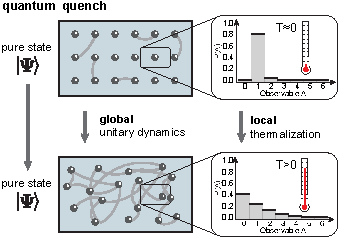
\includegraphics[scale=2]{figures/ETH_fig1.pdf}
	\caption{{\bf Schematic of thermalization dynamics in closed systems}.  An isolated quantum system at zero temperature can be described by a single pure wavefunction $\vert \Psi \rangle$. Subsystems of the full quantum state appear pure, as long as the entanglement (indicated by grey lines) between subsystems is negligible. If suddenly perturbed, the full system evolves unitarily, developing significant entanglement between all parts of the system. While the full system remains in a pure, and in this sense zero-entropy state, the entropy of entanglement causes the subsystems to equilibrate, and local, thermal mixed states appear to emerge within a globally pure quantum state.  }
	\label{fig:conceptual}
\end{figure*}

In the early days of quantum mechanics von Neumann noted that, when talking about thermalization, one should focus on local observables rather then wave functions, who carry all global properties of the system. This approach is very similar to a classical example of isolated container with a gas, where we focus on a small volume inside the container to get a statistical ensemble for the subsystem. From this point of view ETH can be formulated as following: in a quantum chaotic system an expectation value of a local observable is similar between the individual eigenstates and equals to statistical ensemble average. Putting it in more rigorous mathematical terms, ETH states that an expectation value of local observable $O_{nm}$ between eigenstates $\ket{n}$ and $\ket{m}$ is equal to \cite{Srednicki1999}: 
\begin{equation}
O_{nm} = O(\bar{E}) \delta_{nm} + e^{-S(\bar{E})/2} f_O (\bar{E}, \omega) R_{nm},
\end{equation}
where $\bar{E} \equiv (E_n+E_m)/2$, $\omega \equiv E_n-E_m$ and $S(E)$ is thermodynamic entropy at energy $E$. Crucially, $O(E)$ and $f_O(E,ω)$ are smooth functions of their arguments, the value $O(E)$ is identical to the expectation value of the microcanonical ensemble at energy $E$ and $R_{mn}$ is a random real or complex variable with zero mean and unit variance. One important remarks should be made at this point: there are obvious exception form this rule, namely ground state and low lying eigenstates as well as the states on top of the spectrum. Taking this into account, we say that ETH holds for the eigenstates in the middle of the spectrum. 

\subsection{Quench dynamics of an isolated quantum system}
